% TU Delft Beamer template
% Author: Maarten Abbink
% Delft University of Technology
% March 2014
% Version 2.0
% Based on original version 1.0 of Carl Schneider
\documentclass{beamer}
\usepackage[english]{babel}
\usepackage{calc}
\usepackage[absolute,overlay]{textpos}
\mode<presentation>{\usetheme{tud}}

\title[3D folding MaCe]{Guided Three-Dimensional Catalyst Folding during Metal-Assisted Chemical Etching of Silicon}
\institute[TU Delft]{Delft University of Technology}
\author{Dani\"{e}l Bouman}
\date{\today}

% Insert frame before each subsection (requires 2 latex runs)
\AtBeginSubsection[] {
	\begin{frame}<beamer>\frametitle{\titleSubsec}
		\tableofcontents[currentsection,currentsubsection]  % Generation of the Table of Contents
	\end{frame}
}
% Define the title of each inserted pre-subsction frame
\newcommand*\titleSubsec{Next Subsection}
% Define the title of the "Table of Contents" frame
\newcommand*\titleTOC{Outline}

% define a symbol which can be removed if you don't need it
\newcommand{\field}[1]{\mathbb{#1}}
\newcommand{\Zset}{\field{Z}}

\begin{document}

{
% remove the next line if you don't want a background image
\usebackgroundtemplate{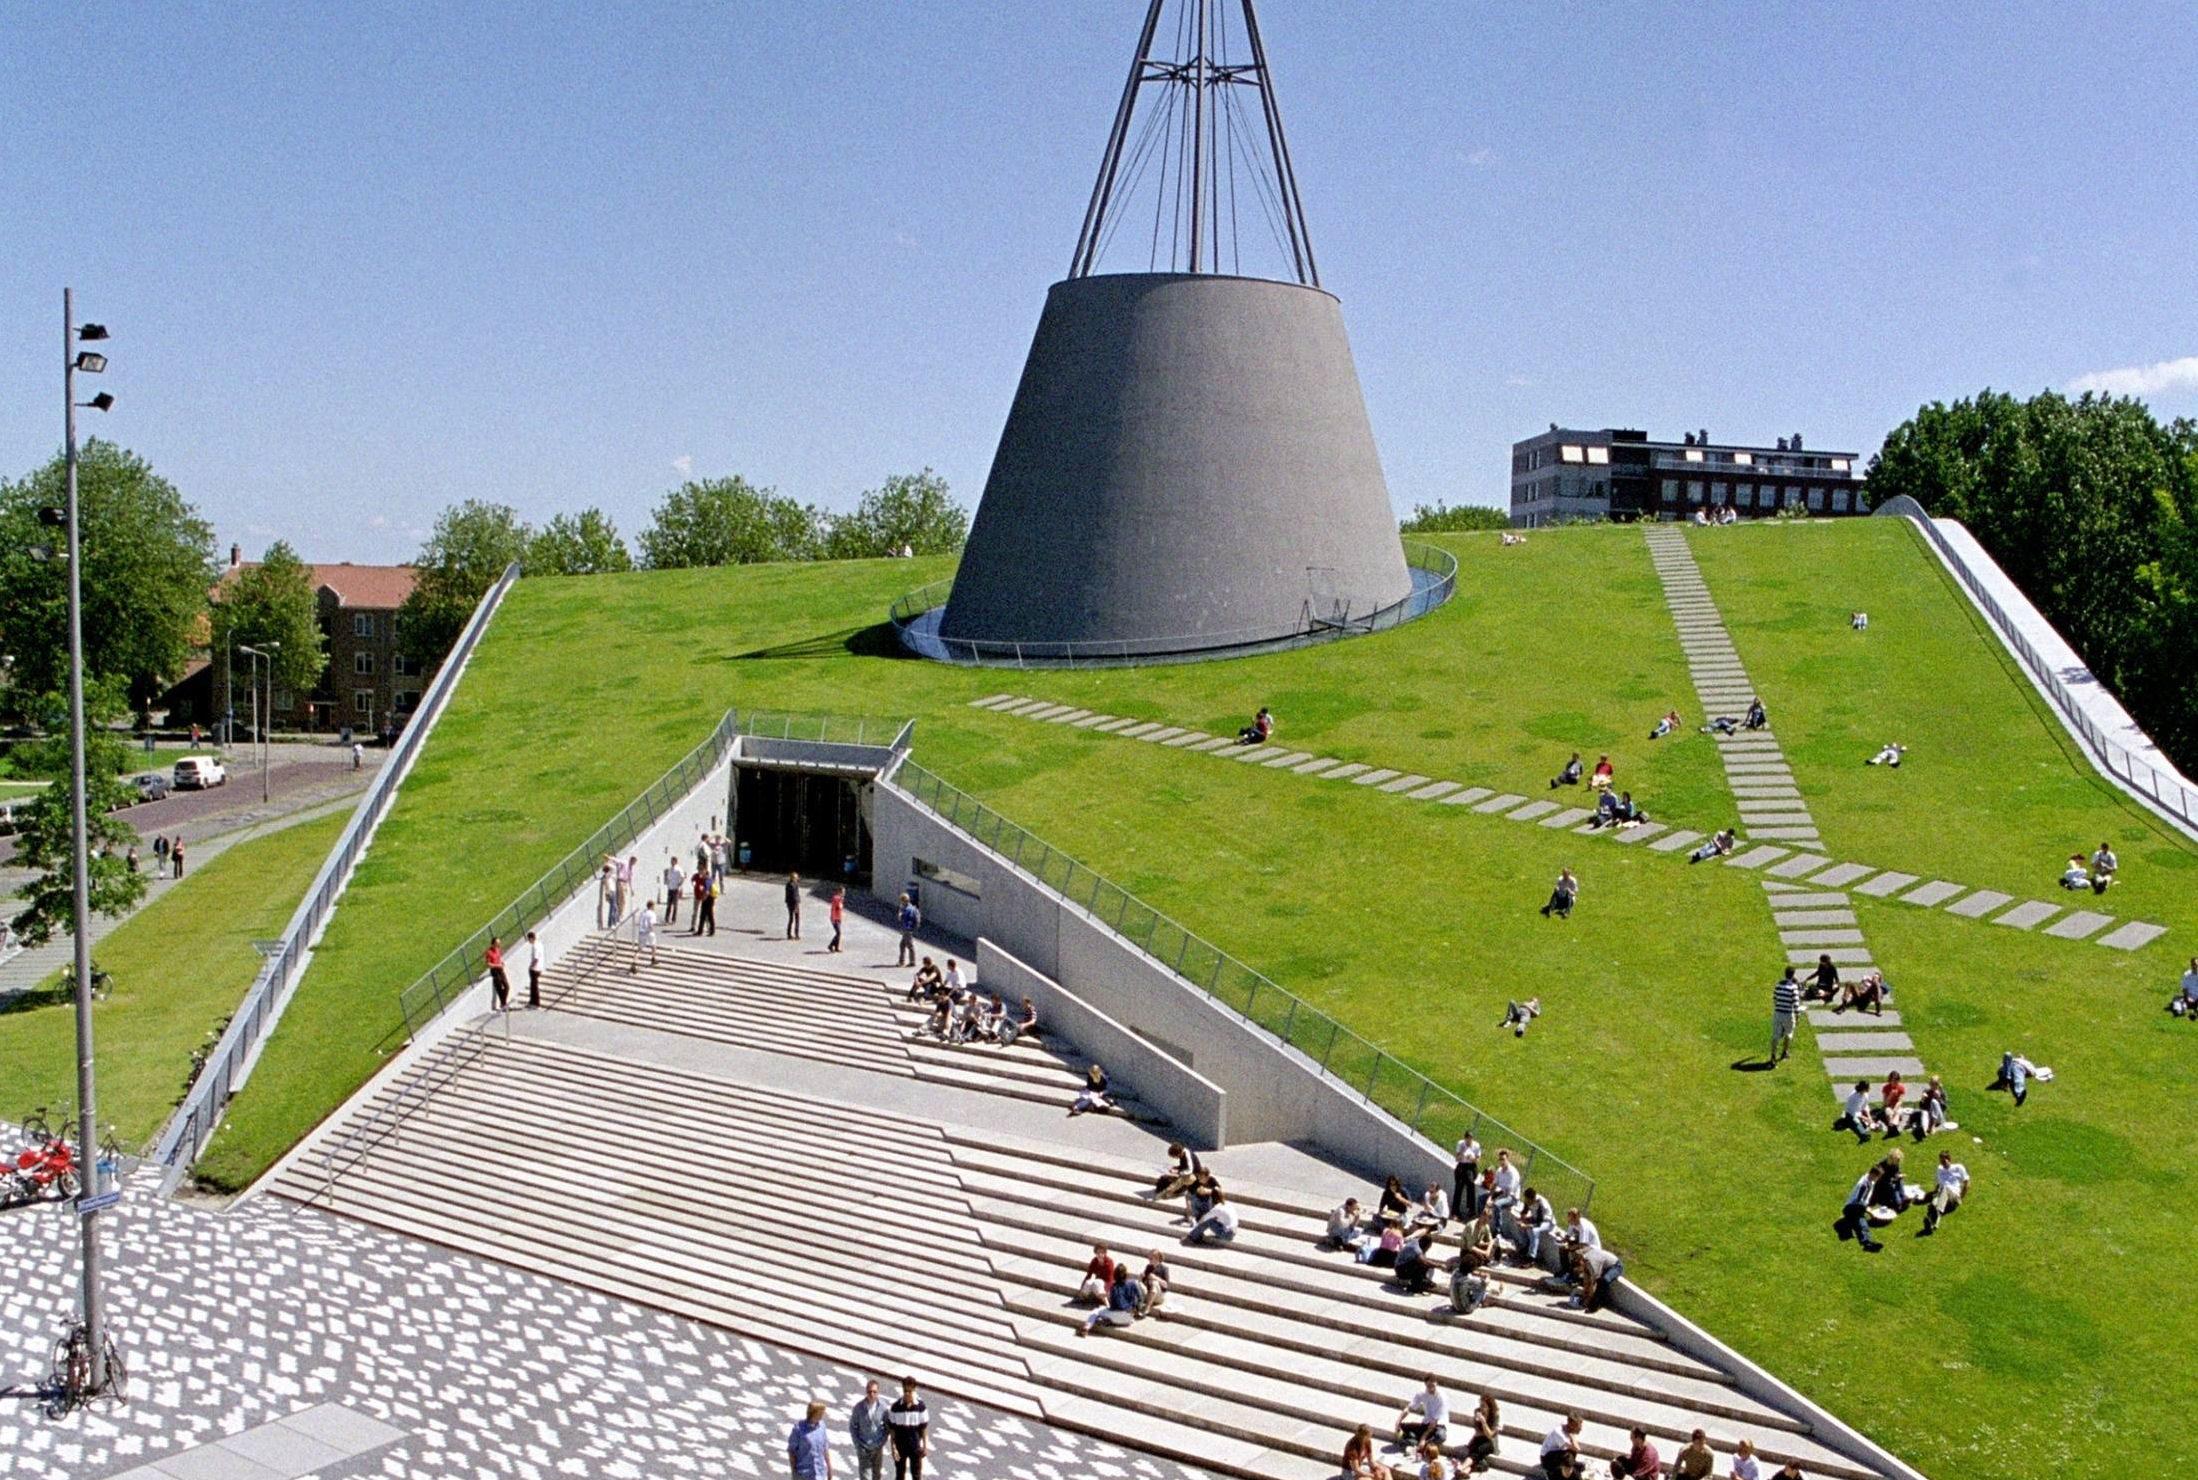
\includegraphics[width=\paperwidth,height=\paperheight]{images/background-titlepage.jpg}}%
\setbeamertemplate{footline}{\usebeamertemplate*{minimal footline}}
\frame{\titlepage}
}

{\setbeamertemplate{footline}{\usebeamertemplate*{minimal footline}}
%\begin{frame}\frametitle{\titleTOC}
%	\tableofcontents
%\end{frame}
}
\begin{frame}\frametitle{Applications of silicon nanostructures}
	\begin{itemize}
	    \item Electronic devices (e.g. Field-effect transistors)
	    \item Batteries
	    \item Thermoelectric devices
	    \item Biochemical sensors
	    \item Photovoltaic cells
	\end{itemize}
\end{frame}

\begin{frame}\frametitle{Traditional methods for creating 3D structures}
    \begin{itemize}
        \item Bottom-up metal catalyzed vapor-liquid-solid (VLS) growth
        \item Top-down lithographic and etching methods
    \end{itemize}
\end{frame}

\begin{frame}\frametitle{Metal-assisted chemical etching (MaCE)}
	\begin{itemize}
	    \item Apply metal catalyst (Au, Ag, Pt) nanoparticles or film onto substrate (often Si)
	    \item Expose to a solution containing redox mediators H$_2$O$_2$ and HF.
	    \item The H$_2$O$_2$ gains electrons (reduction), which creates a cathode at the solution-metal interface.
	    \item This results in a hole-enriched region of Si underneath the metal.
	    \item The holes are consumed at the HF/Si interface producing soluble SiF$_6^2$ and H$_2$SiF$_6$.
	    \item The catalyst travels into the region where the Si was removed.
	\end{itemize}
\end{frame}

\begin{frame}\frametitle{MaCe method}
    \centering
    \begin{minipage}{0.5\textwidth}
		% insert picture (pdf file)
		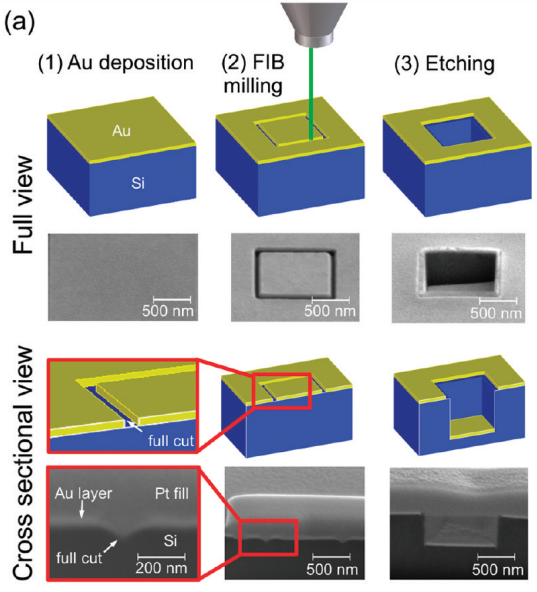
\includegraphics[width=\textwidth]{images/fig1.png}
	\end{minipage}
\end{frame}

\begin{frame}\frametitle{Cross cuts}
    \centering
    \begin{minipage}{0.8\textwidth}
		% insert picture (pdf file)
		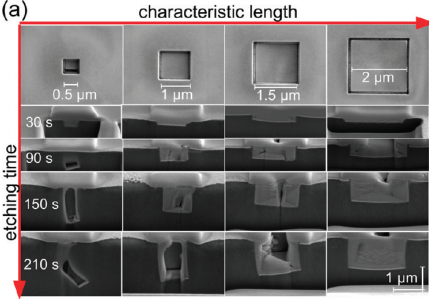
\includegraphics[width=\textwidth]{images/fig2.png}
	\end{minipage}
\end{frame}

\begin{frame}\frametitle{Cross cuts}
    \centering
    \begin{minipage}{\textwidth}
		% insert picture (pdf file)
		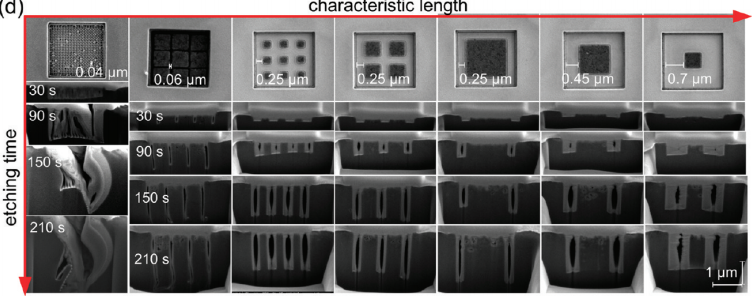
\includegraphics[width=\textwidth]{images/fig3.png}
	\end{minipage}
\end{frame}

\begin{frame}\frametitle{Etch rates}
    \centering
    \begin{minipage}{\textwidth}
		% insert picture (pdf file)
		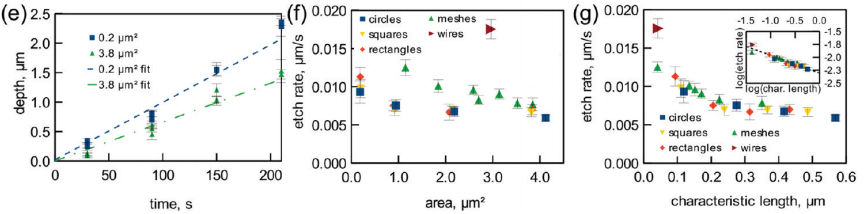
\includegraphics[width=\textwidth]{images/fig4.png}
	\end{minipage}
\end{frame}

\begin{frame}\frametitle{Etch rates}
    The etch rate of MaCe can be controlled by (not limited to)
    \begin{itemize}
        \item Reagent supply to the etch site
        \item Electron and hole transport to the
catalyst surface near the etching interface
        \item Etch product removal
    \end{itemize}
\end{frame}

\begin{frame}\frametitle{Creating hinches}
    \centering
    \begin{minipage}{0.7\textwidth}
		% insert picture (pdf file)
		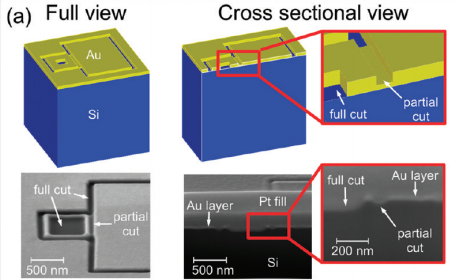
\includegraphics[width=\textwidth]{images/fig5.png}
	\end{minipage}
\end{frame}
\begin{frame}\frametitle{3D folding}
    \centering
    \begin{minipage}{0.7\textwidth}
		% insert picture (pdf file)
		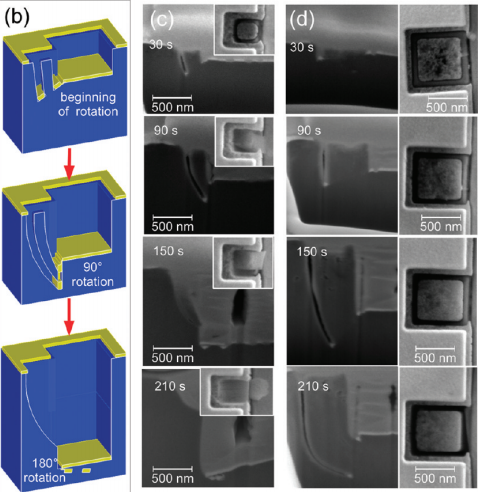
\includegraphics[width=\textwidth]{images/fig6.png}
	\end{minipage}
\end{frame}
\begin{frame}\frametitle{3D folding}
    \centering
    \begin{minipage}{0.7\textwidth}
		% insert picture (pdf file)
		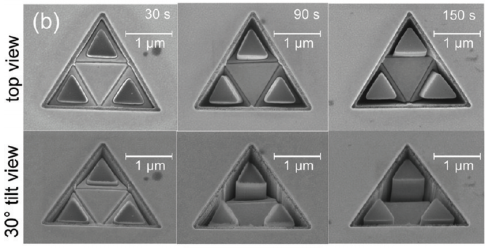
\includegraphics[width=\textwidth]{images/fig8.png}
	\end{minipage}
\end{frame}
\begin{frame}\frametitle{3D folding}
    \centering
    \begin{minipage}{0.5\textwidth}
		% insert picture (pdf file)
		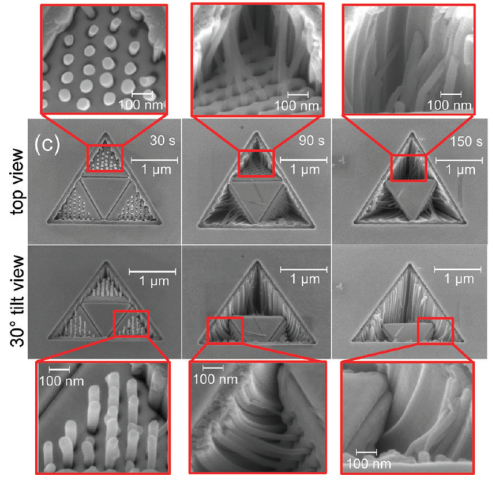
\includegraphics[width=\textwidth]{images/fig7.png}
	\end{minipage}
\end{frame}


\begin{frame}\frametitle{Thank you}
		\centering{Questions?}
\end{frame}

\end{document}
